	\documentclass[titlepage, a4paper]{article}
\usepackage[swedish]{babel}
\usepackage[utf8]{inputenc}
\usepackage{color}
\usepackage{graphicx}
\usepackage{etoolbox}
\usepackage{stringenc}
\usepackage{pdfescape}

% Sidformat
\usepackage{a4wide}

% Fixa Appendix-titlar
\usepackage[titletoc,title]{appendix}

% Bättre tabeller
\usepackage{tabularx}

% Bättre bildtexter
\usepackage[margin=10pt,font=small,labelfont=bf,labelsep=endash]{caption}

% Enkelt kommando som låter mig attgöra-markera text
\newcommand{\todo}[1] {\textbf{\textcolor{red}{#1}}}

% Nytt \paragraph låter oss ha onumrerade bitar
\makeatletter
\renewcommand\paragraph{\@startsection{paragraph}{4}{\z@}%
{-3.25ex\@plus -1ex \@minus -.2ex}%
{1.5ex \@plus .2ex}%
{\normalfont\normalsize\bfseries}}
\makeatother

\providecommand{\LIPSlogga}{../mall/logga1.png}
\providecommand{\LIPSdatum}{\today}

%% Headers och Footers
\usepackage{fancyhdr}
\pagestyle{fancy}
\lhead{\includegraphics[scale=0.4]{\LIPSlogga}}
\rhead{\ifdef{\LIPSutfardare}{Utfärdat av \LIPSutfardare \\\LIPSdatum}\LIPSdatum}
\lfoot{\LIPSkursnamn \\ \LIPSdokumenttyp}
\cfoot{\thepage}
\rfoot{\LIPSprojektgrupp \\ \LIPSprojektnamn}

%% Titelsida
\newcommand{\LIPSTitelsida}{%
{\ }\vspace{45mm}
\begin{center}
  \textbf{\Huge \LIPSdokument}
\end{center}
\begin{center}
  {\Large Redaktör: \LIPSredaktor}
\end{center}
\begin{center}
  {\Large \textbf{Version \LIPSversion}}
\end{center}
\vfill
\begin{center}
  {\large Status}\\[1.5ex]
  \begin{tabular}{|*{3}{p{40mm}|}}
    \hline
    Granskad & \LIPSgranskare & \LIPSgranskatdatum \\
    \hline
    Godkänd & \LIPSgodkannare & \LIPSgodkantdatum \\
    \hline
  \end{tabular}
\end{center}
\newpage
}

% Projektidentitet
\newenvironment{LIPSprojektidentitet}{%
{\ }\vspace{45mm}
\begin{center}
  {\Large PROJEKTIDENTITET}\\[0.5ex]
  {\small
  \LIPSartaltermin, \LIPSprojektgrupp\\
  Linköpings Tekniska Högskola, IDA
  }
\end{center}
\begin{center}
  {\normalsize Gruppdeltagare}\\
  \begin{tabular}{|l|l|p{25mm}|l|}
    \hline
    \textbf{Namn} & \textbf{Ansvar} & \textbf{Telefon} & \textbf{E-post} \\
    \hline
}%
{%
    \hline
  \end{tabular}
\end{center}
\begin{center}
  {\small
    \ifdef{\LIPSgruppadress}{\textbf{E-postlista för hela gruppen}: \LIPSgruppadress\\}{}
    \ifdef{\LIPSgrupphemsida}{\textbf{Hemsida}: \LIPSgrupphemsida\\[1ex]}{}
    \ifdef{\LIPSkund}{\textbf{Kund}: \LIPSkund\\}{}
    \ifdef{\LIPSkundkontakt}{\textbf{Kontaktperson hos kund}: \LIPSkundkontakt\\}{}
    \ifdef{\LIPSkursansvarig}{\textbf{Kursansvarig}: \LIPSkursansvarig\\}{}
    \ifdef{\LIPShandledare}{\textbf{Handledare}: \LIPShandledare\\}{}
  }
\end{center}
\newpage
}
\newcommand{\LIPSgruppmedlem}[4]{\hline {#1} & {#2} & {#3} & {#4} \\}

%% Dokumenthistorik
\newenvironment{LIPSdokumenthistorik}{%
\begin{center}
  Dokumenthistorik\\[1ex]
  %\begin{small}
    \begin{tabular}{|l|l|p{60mm}|l|l|}
      \hline
      \textbf{Version} & \textbf{Datum} & \textbf{Utförda förändringar} & \textbf{Utförda av} & \textbf{Granskad} \\
      }%
    {%
			\hline
    \end{tabular}
  %\end{small}
\end{center}
}

\newcommand{\LIPSversionsinfo}[5]{\hline {#1} & {#2} & {#3} & {#4} & {#5} \\}

% Kravlistor
\newenvironment{LIPSkravlista}{
	\center
		\tabularx{\textwidth}{| p{1.2cm} | p{1.9cm} | X | c |}
			\hline
			\textbf{Krav} & \textbf{Förändring} & \textbf{Beskrivning} & \textbf{Prioritet} \\\hline
}
{
		\endtabularx
	\endcenter
}

\newcounter{LIPSkravnummer}
\addtocounter{LIPSkravnummer}{1}
\newcommand{\LIPSkrav}[4][Krav \arabic{LIPSkravnummer}]{{#1} & {#2} & {#3} & {#4} \stepcounter{LIPSkravnummer}\\\hline}


% Leveranskravlistor
\newenvironment{LIPSleveranskravlista}{
	\center
		\tabularx{\textwidth}{| p{1.2cm} | p{1.9cm} | X | X |}
			\hline
			\textbf{Krav} & \textbf{Förändring} & \textbf{Beskrivning} & \textbf{Deadline}\\\hline
}
{
		\endtabularx
	\endcenter
}

\newcounter{LIPSleveranskravnummer}
\addtocounter{LIPSleveranskravnummer}{1}
\newcommand{\LIPSleveranskrav}[4][Krav \arabic{LIPSkravnummer}]{{#1} & {#2} & {#3} & {#4} \stepcounter{LIPSkravnummer}\\\hline}


% Milstolps-lista
\newenvironment{LIPSmilstolpar}{
	\center
		\tabularx{\textwidth}{| p{1.2cm} | X | l |}
			\hline
			\textbf{Nr} & \textbf{Beskrivning} & \textbf{Datum} \\\hline
}
{
		\endtabularx
	\endcenter
}

\newcounter{LIPSstolpnummer}
\addtocounter{LIPSstolpnummer}{1}
%\newcommand{\LIPSmilstolpe}[3][Krav \arabic{LIPSstolpnummer}]{{#1} & {#2} & {#3} \stepcounter{LIPSstolpnummer}\\\hline}
\newcommand{\LIPSmilstolpe}[3]{{#1} & {#2} & {#3} \\\hline}

% Aktivitets-lista
\newenvironment{LIPSaktivitetslista}{
	\center
		\tabularx{\textwidth}{| p{0.3cm} | X | c | c | c |}
			\hline
			\textbf{Nr} & \textbf{Beskrivning} & \textbf{Beroende av} & \textbf{Timmar} & \textbf{datum} \\\hline
}
{
		\endtabularx
	\endcenter
}

\newcounter{LIPSaktivitetsnummer}
\addtocounter{LIPSaktivitetsnummer}{1}
% \newcommand{\LIPSaktivitet}[4][\arabic{LIPSstolpnummer}]{{#1} & {#2} & {#3} & {#4} \stepcounter{LIPSstolpnummer}\\\hline}
\newcommand{\LIPSaktivitet}[5]{{#1} & {#2} & {#3} & {#4} & {#5}\\\hline}

% Mall för mötesprotokoll
\newenvironment{projektmote}[2]{
  {\ }\vspace{5mm}

  \centerline{\textbf{\Huge #1}}
  \vspace{2mm}
  \centerline{\LARGE #2}
  \vspace{10mm}

  \begin{itemize}
}
{
  \end{itemize}
}

\newcounter{paragrafnummer}
\addtocounter{paragrafnummer}{1}
\newcommand{\paragraf}[1]{\item{\textsection \arabic{paragrafnummer}. {#1}}\addtocounter{paragrafnummer}{1}}

% Mall för Statusrapport
\newenvironment{statusrapport}{
  \center
    \tabularx{\textwidth}{| p{0.4cm} | X | X | p{14.5mm} | p{13.5mm} | p{16.5mm} | p{16.5mm} |}
    \hline
    \textbf{Nr} & \textbf{Aktivitet} & \textbf{Beroenden} & \textbf{Planerad tid} & \textbf{Nedlagd tid} & \textbf{Planerad klar} & \textbf{Beräknat klart} \\\hline
}
{
    \endtabularx
  \endcenter
}

\newcommand{\aktivitetstatus}[7]{{#1} & {#2} & {#3} & {#4} & {#5} & {#6} & {#7} \\\hline}	% Importera generella layout-strukturer

% Information nödvändig för generella layout-strukturer
\newcommand{\LIPSredaktor}{Dennis Ljung}
\newcommand{\LIPSversion}{0.1}
\newcommand{\LIPSdokument}{Projektplan}
\newcommand{\LIPSdokumenttyp}{Projektplan}
\newcommand{\LIPSgranskatdatum}{-}
\newcommand{\LIPSgranskare}{Andreas Runfalk}
\newcommand{\LIPSgodkannare}{Andreas Runfalk}
\newcommand{\LIPSgodkantdatum}{-}
\newcommand{\LIPSkursnamn}{TDDD77}
\newcommand{\LIPSprojektnamn}{Prediktionsreglering}
\newcommand{\LIPSprojektgrupp}{Grupp 2}
%\newcommand{\LIPSgruppadress}{\todo{Ta bort}}
\newcommand{\LIPSartaltermin}{VT, 2015}
\newcommand{\LIPSgrupphemsida}{http://pum-2.ida.liu.se/}
\newcommand{\LIPSkund}{SAAB}
\newcommand{\LIPSkundkontakt}{Daniel Simon}
\newcommand{\LIPSkursansvarig}{Kristian Sandahl}
\newcommand{\LIPShandledare}{Andreas Runfalk}

% Dokument-specifika paket
\usepackage{tabularx}
\usepackage{pdfpages}
\usepackage{tikz}
\usepackage{float}
\usetikzlibrary{shapes, arrows}

\pagenumbering{roman}


\DeclareGraphicsRule{.0.pdf}{pdf}{*}{}

\begin{document}

\LIPSTitelsida

\begin{LIPSprojektidentitet}
	\LIPSgruppmedlem{Adam Sestorp}{Teamledare}{070 9987270}{adase035@student.liu.se}
	\LIPSgruppmedlem{Dennis Ljung}{Dokumentansvarig}{070 8568148}{denlj069@student.liu.se}
	\LIPSgruppmedlem{Alexander Yngve}{Utvecklingsansvarig}{076 2749762}{aleyn573@student.liu.se}
	\LIPSgruppmedlem{Martin Söderén}{Analysansvarig}{070 8163241}{marso329@student.liu.se}
	\LIPSgruppmedlem{Ruben Das}{Kvalitetssamordnare}{073 7355892}{rubda680@student.liu.se}
	\LIPSgruppmedlem{Sebastian Fast}{Arkitekt}{073 3885208}{sebfa861@student.liu.se}
	\LIPSgruppmedlem{Johan Isaksson}{Testledare}{070 2688785}{johis024@student.liu.se}
\end{LIPSprojektidentitet}

\newpage
\tableofcontents	%Innehållsförteckning
%\listoffigures
%\listoftables

\newpage

\begin{LIPSdokumenthistorik}
\LIPSversionsinfo{0.1}{2015-02-09}{Första utkast}{Dennis}{}
\end{LIPSdokumenthistorik}

\newpage
\pagenumbering{arabic}	%Påbörja sidnumrering

% Inledning, översikt osv

\section{Beställare}

Beställare är SAAB AB med Daniel Simon som kontaktperson.

\section{Översiktlig beskrivning av projektet}


\subsection{Syfte och mål}
Syftet med projektet är att:
\begin{enumerate}
 \item gruppen systematiskt ska integrera sina kunskaper som har förvärvats under studietiden, främst inom programmering och datalogi. 
 \item tillämpa sig  metodkunskaper och ämnesmässiga kunskaper inom datateknik
 \item tillgodogöra sig innehållet i relevant facklitteratur och relatera sitt arbete till den
\end{enumerate}

Målet med projektet är att välja ut en lämplig algoritm som löser kvadratiska optimeringsproblem och sedan implementera den effektivt. Denna implementation ska sedan användas för att lösa prediktionsregleringsproblem åt SAAB. 

\subsection{Leveranser}

%H fungerar inte utan float paketet
\begin{table}[H]
  \centering
    \begin{tabularx}{\textwidth}{| X | l | X | l |}
      \hline
      \textbf{Leverans} & \textbf{Ansvarig} & \textbf{Beskrivning} & \textbf{Färdig} \\
      \hline

      {Projekt och teamledare} & {Adam} & {Projektval och val av teamledare ska vara inlämnat till examinator} & {2015-01-23} \\
            \hline
      {Avtal} & {Adam} & {Kopia på avtal med kunden ska vara påskrivet och inlämnat till examinatorn} & {2015-02-03} \\
      \hline
      {Förstudiedokument} & {Adam} & {Kravspecifikation och projektplan ska vara inlämnade till handledare och opponentgrupp} & {2015-02-16} \\
      \hline
      {Förstudiedokument} & {Ruben} & {Kvalitetsplan ska vara inlämnad till handledare och eventuellt kund} & {2015-02-16} \\
      \hline
      {Förstudiedokument} & {Sebastian} & {Första utkast av arkitektplan ska vara påbörjat} & {2015-02-16} \\
      \hline
      {Förstudiedokument} & {Johan} & {Första utkast av testplan ska vara påbörjat} & {2015-02-16} \\
      \hline
      {Dokument} & {Adam} & {Inlämning av halvtids-dokument till handledare och opponentgrupp} & {2015-03-13} \\
      \hline
      {Rapport} & {Adam} & {Utkast 1 av slutrapporten ska vara inlämnat till handledare och opponentgrupp} & {2015-03-13} \\
      \hline
      {Dokument} & {Adam} & {Dokument för iteration 2 ska vara inlämnade till handledaren} & {2015-04-20} \\
      \hline
      {Rapport} & {Adam} & {Utkast 2 av slutrapporten ska vara inlämnade till handledare opponentgrupp och examinator} & {2015-05-13} \\
      \hline
      {Rapport} & {Adam} & {Slutrapport ska vara färdig och inlämnad till handledare och examinator} & {2015-05-27} \\
      \hline

    \end{tabularx}
  \caption{Projektets leveranser.} \label{dokumentation:tabell}
\end{table}



\subsection{Begränsningar}

Projektet är begränsat till att uppfylla de krav som angetts i kravspecifikationen. De krav i kravspecifikationen som angetts med annan prioritet än 1 kommer endast att genomföras i mån av tid. Det finns även begränsningar på hur många timmar som kan läggas på projektet. Från det att förstudien inleds så får varje gruppmedlem max spendera 300 timmar på projeketet. Utöver detta får det max skilja 10\% mellan medlemmer i nedlagd tid.

\section{Fasplan}
Projektet består av fem faser och Alfa-tillstånden finns med i bilaga B:
\begin{enumerate}
\item Förstudie
\item Iteration 1
\item Iteration 2
\item Iteration 3
\item Redovisning och reservtid
\end{enumerate}

\subsection{Förstudie}
Innan iteration 1 genomförs en förstudie där en  kravspecifikation, en projektplan och en kvalitetsplan ska skrivas och lämnas in till handledaren. 

\subsection{Under iterationerna}

Under projektets gång skall handledaren kontinuerligt uppdateras hur projektet fortskrider genom tidsrapporter varje vecka. I slutet av varje iteration ska diverse dokument lämnas in för att ge intressenter en insikt i hur arbetet fortskrider. Även en statusrapport ska kunna skickas iväg till handledare eller kund om det begärs. 


\subsection{Efter projektet}
Efter iteration 3 ska resultatet granskas vid en opponering där projeketet både blir granskat och där gruppen opponerar mot ett annat projekt. Sedan följer en inlämning av en slutrapport, en demonstration av resultatet och överlämning till beställaren. 


\section{Organisationsplan för hela projektet}
Beställaren har beställt projektet från gruppen. Projektledaren är den medlem i gruppen som agerar mellanhand mellan projektgruppen och beställaren. Varje medlem i projektgruppen har ett ansvarsområde där han eller hon leder en arbetsgrupp bestående av delar av resten av gruppen. Det innebär att varje medlem är både arbetsledare och del i minst ett annat arbetslag. En handledare och en grupp tekniska experter finns tillgängliga om gruppen behöver hjälp att lösa något specifikt problem. Figur \ref{projektplan:organisationsplan} illustrerar strukturen.

\begin{figure}[h!]
\center
\tikzset{every picture/.style={scale=0.6}}%
% Graphic for TeX using PGF
% Title: /home/martin/TDDD77/dokumentation/projektplan/grafik/projektplan-organisationsplan.dia
% Creator: Dia v0.97.2
% CreationDate: Tue Feb 10 14:59:02 2015
% For: martin
% \usepackage{tikz}
% The following commands are not supported in PSTricks at present
% We define them conditionally, so when they are implemented,
% this pgf file will use them.
\ifx\du\undefined
  \newlength{\du}
\fi
\setlength{\du}{15\unitlength}
\begin{tikzpicture}
\pgftransformxscale{1.000000}
\pgftransformyscale{-1.000000}
\definecolor{dialinecolor}{rgb}{0.000000, 0.000000, 0.000000}
\pgfsetstrokecolor{dialinecolor}
\definecolor{dialinecolor}{rgb}{1.000000, 1.000000, 1.000000}
\pgfsetfillcolor{dialinecolor}
\pgfsetlinewidth{0.100000\du}
\pgfsetdash{}{0pt}
\pgfsetdash{}{0pt}
\pgfsetbuttcap
\pgfsetmiterjoin
\pgfsetlinewidth{0.100000\du}
\pgfsetbuttcap
\pgfsetmiterjoin
\pgfsetdash{}{0pt}
\definecolor{dialinecolor}{rgb}{1.000000, 1.000000, 1.000000}
\pgfsetfillcolor{dialinecolor}
\pgfpathmoveto{\pgfpoint{28.755625\du}{9.000000\du}}
\pgfpathlineto{\pgfpoint{35.455625\du}{9.000000\du}}
\pgfpathcurveto{\pgfpoint{36.380702\du}{9.000000\du}}{\pgfpoint{37.130625\du}{9.604415\du}}{\pgfpoint{37.130625\du}{10.350000\du}}
\pgfpathcurveto{\pgfpoint{37.130625\du}{11.095585\du}}{\pgfpoint{36.380702\du}{11.700000\du}}{\pgfpoint{35.455625\du}{11.700000\du}}
\pgfpathlineto{\pgfpoint{28.755625\du}{11.700000\du}}
\pgfpathcurveto{\pgfpoint{27.830548\du}{11.700000\du}}{\pgfpoint{27.080625\du}{11.095585\du}}{\pgfpoint{27.080625\du}{10.350000\du}}
\pgfpathcurveto{\pgfpoint{27.080625\du}{9.604415\du}}{\pgfpoint{27.830548\du}{9.000000\du}}{\pgfpoint{28.755625\du}{9.000000\du}}
\pgfusepath{fill}
\definecolor{dialinecolor}{rgb}{0.000000, 0.000000, 0.000000}
\pgfsetstrokecolor{dialinecolor}
\pgfpathmoveto{\pgfpoint{28.755625\du}{9.000000\du}}
\pgfpathlineto{\pgfpoint{35.455625\du}{9.000000\du}}
\pgfpathcurveto{\pgfpoint{36.380702\du}{9.000000\du}}{\pgfpoint{37.130625\du}{9.604415\du}}{\pgfpoint{37.130625\du}{10.350000\du}}
\pgfpathcurveto{\pgfpoint{37.130625\du}{11.095585\du}}{\pgfpoint{36.380702\du}{11.700000\du}}{\pgfpoint{35.455625\du}{11.700000\du}}
\pgfpathlineto{\pgfpoint{28.755625\du}{11.700000\du}}
\pgfpathcurveto{\pgfpoint{27.830548\du}{11.700000\du}}{\pgfpoint{27.080625\du}{11.095585\du}}{\pgfpoint{27.080625\du}{10.350000\du}}
\pgfpathcurveto{\pgfpoint{27.080625\du}{9.604415\du}}{\pgfpoint{27.830548\du}{9.000000\du}}{\pgfpoint{28.755625\du}{9.000000\du}}
\pgfusepath{stroke}
% setfont left to latex
\definecolor{dialinecolor}{rgb}{0.000000, 0.000000, 0.000000}
\pgfsetstrokecolor{dialinecolor}
\node at (32.105625\du,10.150000\du){Beställare};
% setfont left to latex
\definecolor{dialinecolor}{rgb}{0.000000, 0.000000, 0.000000}
\pgfsetstrokecolor{dialinecolor}
\node at (32.105625\du,10.950000\du){Kund};
\pgfsetlinewidth{0.100000\du}
\pgfsetdash{}{0pt}
\pgfsetdash{}{0pt}
\pgfsetbuttcap
\pgfsetmiterjoin
\pgfsetlinewidth{0.100000\du}
\pgfsetbuttcap
\pgfsetmiterjoin
\pgfsetdash{}{0pt}
\definecolor{dialinecolor}{rgb}{1.000000, 1.000000, 1.000000}
\pgfsetfillcolor{dialinecolor}
\pgfpathmoveto{\pgfpoint{10.878125\du}{35.000000\du}}
\pgfpathlineto{\pgfpoint{18.390625\du}{35.000000\du}}
\pgfpathcurveto{\pgfpoint{19.427885\du}{35.000000\du}}{\pgfpoint{20.268750\du}{35.604415\du}}{\pgfpoint{20.268750\du}{36.350000\du}}
\pgfpathcurveto{\pgfpoint{20.268750\du}{37.095585\du}}{\pgfpoint{19.427885\du}{37.700000\du}}{\pgfpoint{18.390625\du}{37.700000\du}}
\pgfpathlineto{\pgfpoint{10.878125\du}{37.700000\du}}
\pgfpathcurveto{\pgfpoint{9.840865\du}{37.700000\du}}{\pgfpoint{9.000000\du}{37.095585\du}}{\pgfpoint{9.000000\du}{36.350000\du}}
\pgfpathcurveto{\pgfpoint{9.000000\du}{35.604415\du}}{\pgfpoint{9.840865\du}{35.000000\du}}{\pgfpoint{10.878125\du}{35.000000\du}}
\pgfusepath{fill}
\definecolor{dialinecolor}{rgb}{0.000000, 0.000000, 0.000000}
\pgfsetstrokecolor{dialinecolor}
\pgfpathmoveto{\pgfpoint{10.878125\du}{35.000000\du}}
\pgfpathlineto{\pgfpoint{18.390625\du}{35.000000\du}}
\pgfpathcurveto{\pgfpoint{19.427885\du}{35.000000\du}}{\pgfpoint{20.268750\du}{35.604415\du}}{\pgfpoint{20.268750\du}{36.350000\du}}
\pgfpathcurveto{\pgfpoint{20.268750\du}{37.095585\du}}{\pgfpoint{19.427885\du}{37.700000\du}}{\pgfpoint{18.390625\du}{37.700000\du}}
\pgfpathlineto{\pgfpoint{10.878125\du}{37.700000\du}}
\pgfpathcurveto{\pgfpoint{9.840865\du}{37.700000\du}}{\pgfpoint{9.000000\du}{37.095585\du}}{\pgfpoint{9.000000\du}{36.350000\du}}
\pgfpathcurveto{\pgfpoint{9.000000\du}{35.604415\du}}{\pgfpoint{9.840865\du}{35.000000\du}}{\pgfpoint{10.878125\du}{35.000000\du}}
\pgfusepath{stroke}
% setfont left to latex
\definecolor{dialinecolor}{rgb}{0.000000, 0.000000, 0.000000}
\pgfsetstrokecolor{dialinecolor}
\node at (14.634375\du,36.550000\du){Teamleader};
\pgfsetlinewidth{0.100000\du}
\pgfsetdash{}{0pt}
\pgfsetdash{}{0pt}
\pgfsetbuttcap
\pgfsetmiterjoin
\pgfsetlinewidth{0.100000\du}
\pgfsetbuttcap
\pgfsetmiterjoin
\pgfsetdash{}{0pt}
\definecolor{dialinecolor}{rgb}{1.000000, 1.000000, 1.000000}
\pgfsetfillcolor{dialinecolor}
\pgfpathmoveto{\pgfpoint{11.284375\du}{15.046250\du}}
\pgfpathlineto{\pgfpoint{17.984375\du}{15.046250\du}}
\pgfpathcurveto{\pgfpoint{18.909452\du}{15.046250\du}}{\pgfpoint{19.659375\du}{15.629958\du}}{\pgfpoint{19.659375\du}{16.350000\du}}
\pgfpathcurveto{\pgfpoint{19.659375\du}{17.070042\du}}{\pgfpoint{18.909452\du}{17.653750\du}}{\pgfpoint{17.984375\du}{17.653750\du}}
\pgfpathlineto{\pgfpoint{11.284375\du}{17.653750\du}}
\pgfpathcurveto{\pgfpoint{10.359298\du}{17.653750\du}}{\pgfpoint{9.609375\du}{17.070042\du}}{\pgfpoint{9.609375\du}{16.350000\du}}
\pgfpathcurveto{\pgfpoint{9.609375\du}{15.629958\du}}{\pgfpoint{10.359298\du}{15.046250\du}}{\pgfpoint{11.284375\du}{15.046250\du}}
\pgfusepath{fill}
\definecolor{dialinecolor}{rgb}{0.000000, 0.000000, 0.000000}
\pgfsetstrokecolor{dialinecolor}
\pgfpathmoveto{\pgfpoint{11.284375\du}{15.046250\du}}
\pgfpathlineto{\pgfpoint{17.984375\du}{15.046250\du}}
\pgfpathcurveto{\pgfpoint{18.909452\du}{15.046250\du}}{\pgfpoint{19.659375\du}{15.629958\du}}{\pgfpoint{19.659375\du}{16.350000\du}}
\pgfpathcurveto{\pgfpoint{19.659375\du}{17.070042\du}}{\pgfpoint{18.909452\du}{17.653750\du}}{\pgfpoint{17.984375\du}{17.653750\du}}
\pgfpathlineto{\pgfpoint{11.284375\du}{17.653750\du}}
\pgfpathcurveto{\pgfpoint{10.359298\du}{17.653750\du}}{\pgfpoint{9.609375\du}{17.070042\du}}{\pgfpoint{9.609375\du}{16.350000\du}}
\pgfpathcurveto{\pgfpoint{9.609375\du}{15.629958\du}}{\pgfpoint{10.359298\du}{15.046250\du}}{\pgfpoint{11.284375\du}{15.046250\du}}
\pgfusepath{stroke}
% setfont left to latex
\definecolor{dialinecolor}{rgb}{0.000000, 0.000000, 0.000000}
\pgfsetstrokecolor{dialinecolor}
\node at (14.634375\du,16.550000\du){Handledare};
\pgfsetlinewidth{0.100000\du}
\pgfsetdash{}{0pt}
\pgfsetdash{}{0pt}
\pgfsetbuttcap
\pgfsetmiterjoin
\pgfsetlinewidth{0.100000\du}
\pgfsetbuttcap
\pgfsetmiterjoin
\pgfsetdash{}{0pt}
\definecolor{dialinecolor}{rgb}{1.000000, 1.000000, 1.000000}
\pgfsetfillcolor{dialinecolor}
\pgfpathmoveto{\pgfpoint{28.755625\du}{15.000000\du}}
\pgfpathlineto{\pgfpoint{35.455625\du}{15.000000\du}}
\pgfpathcurveto{\pgfpoint{36.380702\du}{15.000000\du}}{\pgfpoint{37.130625\du}{15.604415\du}}{\pgfpoint{37.130625\du}{16.350000\du}}
\pgfpathcurveto{\pgfpoint{37.130625\du}{17.095585\du}}{\pgfpoint{36.380702\du}{17.700000\du}}{\pgfpoint{35.455625\du}{17.700000\du}}
\pgfpathlineto{\pgfpoint{28.755625\du}{17.700000\du}}
\pgfpathcurveto{\pgfpoint{27.830548\du}{17.700000\du}}{\pgfpoint{27.080625\du}{17.095585\du}}{\pgfpoint{27.080625\du}{16.350000\du}}
\pgfpathcurveto{\pgfpoint{27.080625\du}{15.604415\du}}{\pgfpoint{27.830548\du}{15.000000\du}}{\pgfpoint{28.755625\du}{15.000000\du}}
\pgfusepath{fill}
\definecolor{dialinecolor}{rgb}{0.000000, 0.000000, 0.000000}
\pgfsetstrokecolor{dialinecolor}
\pgfpathmoveto{\pgfpoint{28.755625\du}{15.000000\du}}
\pgfpathlineto{\pgfpoint{35.455625\du}{15.000000\du}}
\pgfpathcurveto{\pgfpoint{36.380702\du}{15.000000\du}}{\pgfpoint{37.130625\du}{15.604415\du}}{\pgfpoint{37.130625\du}{16.350000\du}}
\pgfpathcurveto{\pgfpoint{37.130625\du}{17.095585\du}}{\pgfpoint{36.380702\du}{17.700000\du}}{\pgfpoint{35.455625\du}{17.700000\du}}
\pgfpathlineto{\pgfpoint{28.755625\du}{17.700000\du}}
\pgfpathcurveto{\pgfpoint{27.830548\du}{17.700000\du}}{\pgfpoint{27.080625\du}{17.095585\du}}{\pgfpoint{27.080625\du}{16.350000\du}}
\pgfpathcurveto{\pgfpoint{27.080625\du}{15.604415\du}}{\pgfpoint{27.830548\du}{15.000000\du}}{\pgfpoint{28.755625\du}{15.000000\du}}
\pgfusepath{stroke}
% setfont left to latex
\definecolor{dialinecolor}{rgb}{0.000000, 0.000000, 0.000000}
\pgfsetstrokecolor{dialinecolor}
\node at (32.105625\du,16.550000\du){Analysansvarig};
\pgfsetlinewidth{0.100000\du}
\pgfsetdash{}{0pt}
\pgfsetdash{}{0pt}
\pgfsetbuttcap
\pgfsetmiterjoin
\pgfsetlinewidth{0.100000\du}
\pgfsetbuttcap
\pgfsetmiterjoin
\pgfsetdash{}{0pt}
\definecolor{dialinecolor}{rgb}{1.000000, 1.000000, 1.000000}
\pgfsetfillcolor{dialinecolor}
\pgfpathmoveto{\pgfpoint{28.755625\du}{19.000000\du}}
\pgfpathlineto{\pgfpoint{35.455625\du}{19.000000\du}}
\pgfpathcurveto{\pgfpoint{36.380702\du}{19.000000\du}}{\pgfpoint{37.130625\du}{19.604415\du}}{\pgfpoint{37.130625\du}{20.350000\du}}
\pgfpathcurveto{\pgfpoint{37.130625\du}{21.095585\du}}{\pgfpoint{36.380702\du}{21.700000\du}}{\pgfpoint{35.455625\du}{21.700000\du}}
\pgfpathlineto{\pgfpoint{28.755625\du}{21.700000\du}}
\pgfpathcurveto{\pgfpoint{27.830548\du}{21.700000\du}}{\pgfpoint{27.080625\du}{21.095585\du}}{\pgfpoint{27.080625\du}{20.350000\du}}
\pgfpathcurveto{\pgfpoint{27.080625\du}{19.604415\du}}{\pgfpoint{27.830548\du}{19.000000\du}}{\pgfpoint{28.755625\du}{19.000000\du}}
\pgfusepath{fill}
\definecolor{dialinecolor}{rgb}{0.000000, 0.000000, 0.000000}
\pgfsetstrokecolor{dialinecolor}
\pgfpathmoveto{\pgfpoint{28.755625\du}{19.000000\du}}
\pgfpathlineto{\pgfpoint{35.455625\du}{19.000000\du}}
\pgfpathcurveto{\pgfpoint{36.380702\du}{19.000000\du}}{\pgfpoint{37.130625\du}{19.604415\du}}{\pgfpoint{37.130625\du}{20.350000\du}}
\pgfpathcurveto{\pgfpoint{37.130625\du}{21.095585\du}}{\pgfpoint{36.380702\du}{21.700000\du}}{\pgfpoint{35.455625\du}{21.700000\du}}
\pgfpathlineto{\pgfpoint{28.755625\du}{21.700000\du}}
\pgfpathcurveto{\pgfpoint{27.830548\du}{21.700000\du}}{\pgfpoint{27.080625\du}{21.095585\du}}{\pgfpoint{27.080625\du}{20.350000\du}}
\pgfpathcurveto{\pgfpoint{27.080625\du}{19.604415\du}}{\pgfpoint{27.830548\du}{19.000000\du}}{\pgfpoint{28.755625\du}{19.000000\du}}
\pgfusepath{stroke}
% setfont left to latex
\definecolor{dialinecolor}{rgb}{0.000000, 0.000000, 0.000000}
\pgfsetstrokecolor{dialinecolor}
\node at (32.105625\du,20.550000\du){Arkitekt};
\pgfsetlinewidth{0.100000\du}
\pgfsetdash{}{0pt}
\pgfsetdash{}{0pt}
\pgfsetbuttcap
\pgfsetmiterjoin
\pgfsetlinewidth{0.100000\du}
\pgfsetbuttcap
\pgfsetmiterjoin
\pgfsetdash{}{0pt}
\definecolor{dialinecolor}{rgb}{1.000000, 1.000000, 1.000000}
\pgfsetfillcolor{dialinecolor}
\pgfpathmoveto{\pgfpoint{28.755625\du}{23.000000\du}}
\pgfpathlineto{\pgfpoint{35.455625\du}{23.000000\du}}
\pgfpathcurveto{\pgfpoint{36.380702\du}{23.000000\du}}{\pgfpoint{37.130625\du}{23.604415\du}}{\pgfpoint{37.130625\du}{24.350000\du}}
\pgfpathcurveto{\pgfpoint{37.130625\du}{25.095585\du}}{\pgfpoint{36.380702\du}{25.700000\du}}{\pgfpoint{35.455625\du}{25.700000\du}}
\pgfpathlineto{\pgfpoint{28.755625\du}{25.700000\du}}
\pgfpathcurveto{\pgfpoint{27.830548\du}{25.700000\du}}{\pgfpoint{27.080625\du}{25.095585\du}}{\pgfpoint{27.080625\du}{24.350000\du}}
\pgfpathcurveto{\pgfpoint{27.080625\du}{23.604415\du}}{\pgfpoint{27.830548\du}{23.000000\du}}{\pgfpoint{28.755625\du}{23.000000\du}}
\pgfusepath{fill}
\definecolor{dialinecolor}{rgb}{0.000000, 0.000000, 0.000000}
\pgfsetstrokecolor{dialinecolor}
\pgfpathmoveto{\pgfpoint{28.755625\du}{23.000000\du}}
\pgfpathlineto{\pgfpoint{35.455625\du}{23.000000\du}}
\pgfpathcurveto{\pgfpoint{36.380702\du}{23.000000\du}}{\pgfpoint{37.130625\du}{23.604415\du}}{\pgfpoint{37.130625\du}{24.350000\du}}
\pgfpathcurveto{\pgfpoint{37.130625\du}{25.095585\du}}{\pgfpoint{36.380702\du}{25.700000\du}}{\pgfpoint{35.455625\du}{25.700000\du}}
\pgfpathlineto{\pgfpoint{28.755625\du}{25.700000\du}}
\pgfpathcurveto{\pgfpoint{27.830548\du}{25.700000\du}}{\pgfpoint{27.080625\du}{25.095585\du}}{\pgfpoint{27.080625\du}{24.350000\du}}
\pgfpathcurveto{\pgfpoint{27.080625\du}{23.604415\du}}{\pgfpoint{27.830548\du}{23.000000\du}}{\pgfpoint{28.755625\du}{23.000000\du}}
\pgfusepath{stroke}
% setfont left to latex
\definecolor{dialinecolor}{rgb}{0.000000, 0.000000, 0.000000}
\pgfsetstrokecolor{dialinecolor}
\node at (32.105625\du,24.550000\du){Dokumentansvarig};
\pgfsetlinewidth{0.100000\du}
\pgfsetdash{}{0pt}
\pgfsetdash{}{0pt}
\pgfsetbuttcap
\pgfsetmiterjoin
\pgfsetlinewidth{0.100000\du}
\pgfsetbuttcap
\pgfsetmiterjoin
\pgfsetdash{}{0pt}
\definecolor{dialinecolor}{rgb}{1.000000, 1.000000, 1.000000}
\pgfsetfillcolor{dialinecolor}
\pgfpathmoveto{\pgfpoint{28.723125\du}{27.000000\du}}
\pgfpathlineto{\pgfpoint{35.488125\du}{27.000000\du}}
\pgfpathcurveto{\pgfpoint{36.422177\du}{27.000000\du}}{\pgfpoint{37.179375\du}{27.604415\du}}{\pgfpoint{37.179375\du}{28.350000\du}}
\pgfpathcurveto{\pgfpoint{37.179375\du}{29.095585\du}}{\pgfpoint{36.422177\du}{29.700000\du}}{\pgfpoint{35.488125\du}{29.700000\du}}
\pgfpathlineto{\pgfpoint{28.723125\du}{29.700000\du}}
\pgfpathcurveto{\pgfpoint{27.789073\du}{29.700000\du}}{\pgfpoint{27.031875\du}{29.095585\du}}{\pgfpoint{27.031875\du}{28.350000\du}}
\pgfpathcurveto{\pgfpoint{27.031875\du}{27.604415\du}}{\pgfpoint{27.789073\du}{27.000000\du}}{\pgfpoint{28.723125\du}{27.000000\du}}
\pgfusepath{fill}
\definecolor{dialinecolor}{rgb}{0.000000, 0.000000, 0.000000}
\pgfsetstrokecolor{dialinecolor}
\pgfpathmoveto{\pgfpoint{28.723125\du}{27.000000\du}}
\pgfpathlineto{\pgfpoint{35.488125\du}{27.000000\du}}
\pgfpathcurveto{\pgfpoint{36.422177\du}{27.000000\du}}{\pgfpoint{37.179375\du}{27.604415\du}}{\pgfpoint{37.179375\du}{28.350000\du}}
\pgfpathcurveto{\pgfpoint{37.179375\du}{29.095585\du}}{\pgfpoint{36.422177\du}{29.700000\du}}{\pgfpoint{35.488125\du}{29.700000\du}}
\pgfpathlineto{\pgfpoint{28.723125\du}{29.700000\du}}
\pgfpathcurveto{\pgfpoint{27.789073\du}{29.700000\du}}{\pgfpoint{27.031875\du}{29.095585\du}}{\pgfpoint{27.031875\du}{28.350000\du}}
\pgfpathcurveto{\pgfpoint{27.031875\du}{27.604415\du}}{\pgfpoint{27.789073\du}{27.000000\du}}{\pgfpoint{28.723125\du}{27.000000\du}}
\pgfusepath{stroke}
% setfont left to latex
\definecolor{dialinecolor}{rgb}{0.000000, 0.000000, 0.000000}
\pgfsetstrokecolor{dialinecolor}
\node at (32.105625\du,28.550000\du){Utvecklingsansvarig};
\pgfsetlinewidth{0.100000\du}
\pgfsetdash{}{0pt}
\pgfsetdash{}{0pt}
\pgfsetbuttcap
\pgfsetmiterjoin
\pgfsetlinewidth{0.100000\du}
\pgfsetbuttcap
\pgfsetmiterjoin
\pgfsetdash{}{0pt}
\definecolor{dialinecolor}{rgb}{1.000000, 1.000000, 1.000000}
\pgfsetfillcolor{dialinecolor}
\pgfpathmoveto{\pgfpoint{28.648125\du}{31.000000\du}}
\pgfpathlineto{\pgfpoint{35.563125\du}{31.000000\du}}
\pgfpathcurveto{\pgfpoint{36.517888\du}{31.000000\du}}{\pgfpoint{37.291875\du}{31.604415\du}}{\pgfpoint{37.291875\du}{32.350000\du}}
\pgfpathcurveto{\pgfpoint{37.291875\du}{33.095585\du}}{\pgfpoint{36.517888\du}{33.700000\du}}{\pgfpoint{35.563125\du}{33.700000\du}}
\pgfpathlineto{\pgfpoint{28.648125\du}{33.700000\du}}
\pgfpathcurveto{\pgfpoint{27.693362\du}{33.700000\du}}{\pgfpoint{26.919375\du}{33.095585\du}}{\pgfpoint{26.919375\du}{32.350000\du}}
\pgfpathcurveto{\pgfpoint{26.919375\du}{31.604415\du}}{\pgfpoint{27.693362\du}{31.000000\du}}{\pgfpoint{28.648125\du}{31.000000\du}}
\pgfusepath{fill}
\definecolor{dialinecolor}{rgb}{0.000000, 0.000000, 0.000000}
\pgfsetstrokecolor{dialinecolor}
\pgfpathmoveto{\pgfpoint{28.648125\du}{31.000000\du}}
\pgfpathlineto{\pgfpoint{35.563125\du}{31.000000\du}}
\pgfpathcurveto{\pgfpoint{36.517888\du}{31.000000\du}}{\pgfpoint{37.291875\du}{31.604415\du}}{\pgfpoint{37.291875\du}{32.350000\du}}
\pgfpathcurveto{\pgfpoint{37.291875\du}{33.095585\du}}{\pgfpoint{36.517888\du}{33.700000\du}}{\pgfpoint{35.563125\du}{33.700000\du}}
\pgfpathlineto{\pgfpoint{28.648125\du}{33.700000\du}}
\pgfpathcurveto{\pgfpoint{27.693362\du}{33.700000\du}}{\pgfpoint{26.919375\du}{33.095585\du}}{\pgfpoint{26.919375\du}{32.350000\du}}
\pgfpathcurveto{\pgfpoint{26.919375\du}{31.604415\du}}{\pgfpoint{27.693362\du}{31.000000\du}}{\pgfpoint{28.648125\du}{31.000000\du}}
\pgfusepath{stroke}
% setfont left to latex
\definecolor{dialinecolor}{rgb}{0.000000, 0.000000, 0.000000}
\pgfsetstrokecolor{dialinecolor}
\node at (32.105625\du,32.550000\du){Kvalitetssamordnare};
\pgfsetlinewidth{0.100000\du}
\pgfsetdash{}{0pt}
\pgfsetdash{}{0pt}
\pgfsetbuttcap
{
\definecolor{dialinecolor}{rgb}{0.000000, 0.000000, 0.000000}
\pgfsetfillcolor{dialinecolor}
% was here!!!
\pgfsetarrowsstart{stealth}
\definecolor{dialinecolor}{rgb}{0.000000, 0.000000, 0.000000}
\pgfsetstrokecolor{dialinecolor}
\draw (27.080625\du,16.350000\du)--(15.505324\du,34.950464\du);
}
\pgfsetlinewidth{0.100000\du}
\pgfsetdash{}{0pt}
\pgfsetdash{}{0pt}
\pgfsetbuttcap
{
\definecolor{dialinecolor}{rgb}{0.000000, 0.000000, 0.000000}
\pgfsetfillcolor{dialinecolor}
% was here!!!
\pgfsetarrowsstart{stealth}
\definecolor{dialinecolor}{rgb}{0.000000, 0.000000, 0.000000}
\pgfsetstrokecolor{dialinecolor}
\draw (27.080625\du,20.350000\du)--(15.722966\du,34.950586\du);
}
\pgfsetlinewidth{0.100000\du}
\pgfsetdash{}{0pt}
\pgfsetdash{}{0pt}
\pgfsetbuttcap
{
\definecolor{dialinecolor}{rgb}{0.000000, 0.000000, 0.000000}
\pgfsetfillcolor{dialinecolor}
% was here!!!
\pgfsetarrowsstart{stealth}
\definecolor{dialinecolor}{rgb}{0.000000, 0.000000, 0.000000}
\pgfsetstrokecolor{dialinecolor}
\draw (27.080625\du,24.350000\du)--(16.083804\du,34.952539\du);
}
\pgfsetlinewidth{0.100000\du}
\pgfsetdash{}{0pt}
\pgfsetdash{}{0pt}
\pgfsetbuttcap
{
\definecolor{dialinecolor}{rgb}{0.000000, 0.000000, 0.000000}
\pgfsetfillcolor{dialinecolor}
% was here!!!
\pgfsetarrowsstart{stealth}
\definecolor{dialinecolor}{rgb}{0.000000, 0.000000, 0.000000}
\pgfsetstrokecolor{dialinecolor}
\draw (27.031875\du,28.350000\du)--(16.803029\du,34.950586\du);
}
\pgfsetlinewidth{0.100000\du}
\pgfsetdash{}{0pt}
\pgfsetdash{}{0pt}
\pgfsetbuttcap
{
\definecolor{dialinecolor}{rgb}{0.000000, 0.000000, 0.000000}
\pgfsetfillcolor{dialinecolor}
% was here!!!
\pgfsetarrowsstart{stealth}
\definecolor{dialinecolor}{rgb}{0.000000, 0.000000, 0.000000}
\pgfsetstrokecolor{dialinecolor}
\draw (26.919375\du,32.350000\du)--(18.816854\du,34.988184\du);
}
\pgfsetlinewidth{0.100000\du}
\pgfsetdash{}{0pt}
\pgfsetdash{}{0pt}
\pgfsetbuttcap
\pgfsetmiterjoin
\pgfsetlinewidth{0.100000\du}
\pgfsetbuttcap
\pgfsetmiterjoin
\pgfsetdash{}{0pt}
\definecolor{dialinecolor}{rgb}{1.000000, 1.000000, 1.000000}
\pgfsetfillcolor{dialinecolor}
\pgfpathmoveto{\pgfpoint{42.991667\du}{25.449997\du}}
\pgfpathlineto{\pgfpoint{51.158334\du}{25.449997\du}}
\pgfpathcurveto{\pgfpoint{52.285916\du}{25.449997\du}}{\pgfpoint{53.200000\du}{25.987255\du}}{\pgfpoint{53.200000\du}{26.649997\du}}
\pgfpathcurveto{\pgfpoint{53.200000\du}{27.312739\du}}{\pgfpoint{52.285916\du}{27.849997\du}}{\pgfpoint{51.158334\du}{27.849997\du}}
\pgfpathlineto{\pgfpoint{42.991667\du}{27.849997\du}}
\pgfpathcurveto{\pgfpoint{41.864085\du}{27.849997\du}}{\pgfpoint{40.950000\du}{27.312739\du}}{\pgfpoint{40.950000\du}{26.649997\du}}
\pgfpathcurveto{\pgfpoint{40.950000\du}{25.987255\du}}{\pgfpoint{41.864085\du}{25.449997\du}}{\pgfpoint{42.991667\du}{25.449997\du}}
\pgfusepath{fill}
\definecolor{dialinecolor}{rgb}{0.000000, 0.000000, 0.000000}
\pgfsetstrokecolor{dialinecolor}
\pgfpathmoveto{\pgfpoint{42.991667\du}{25.449997\du}}
\pgfpathlineto{\pgfpoint{51.158334\du}{25.449997\du}}
\pgfpathcurveto{\pgfpoint{52.285916\du}{25.449997\du}}{\pgfpoint{53.200000\du}{25.987255\du}}{\pgfpoint{53.200000\du}{26.649997\du}}
\pgfpathcurveto{\pgfpoint{53.200000\du}{27.312739\du}}{\pgfpoint{52.285916\du}{27.849997\du}}{\pgfpoint{51.158334\du}{27.849997\du}}
\pgfpathlineto{\pgfpoint{42.991667\du}{27.849997\du}}
\pgfpathcurveto{\pgfpoint{41.864085\du}{27.849997\du}}{\pgfpoint{40.950000\du}{27.312739\du}}{\pgfpoint{40.950000\du}{26.649997\du}}
\pgfpathcurveto{\pgfpoint{40.950000\du}{25.987255\du}}{\pgfpoint{41.864085\du}{25.449997\du}}{\pgfpoint{42.991667\du}{25.449997\du}}
\pgfusepath{stroke}
% setfont left to latex
\definecolor{dialinecolor}{rgb}{0.000000, 0.000000, 0.000000}
\pgfsetstrokecolor{dialinecolor}
\node at (47.075000\du,26.849997\du){Interna arbetsgrupper};
% setfont left to latex
\definecolor{dialinecolor}{rgb}{0.000000, 0.000000, 0.000000}
\pgfsetstrokecolor{dialinecolor}
\node[anchor=west] at (14.634375\du,36.350000\du){};
\pgfsetlinewidth{0.100000\du}
\pgfsetdash{}{0pt}
\pgfsetdash{}{0pt}
\pgfsetbuttcap
{
\definecolor{dialinecolor}{rgb}{0.000000, 0.000000, 0.000000}
\pgfsetfillcolor{dialinecolor}
% was here!!!
\pgfsetarrowsstart{stealth}
\definecolor{dialinecolor}{rgb}{0.000000, 0.000000, 0.000000}
\pgfsetstrokecolor{dialinecolor}
\draw (32.105625\du,14.952539\du)--(32.105625\du,11.747461\du);
}
\pgfsetlinewidth{0.100000\du}
\pgfsetdash{}{0pt}
\pgfsetdash{}{0pt}
\pgfsetbuttcap
{
\definecolor{dialinecolor}{rgb}{0.000000, 0.000000, 0.000000}
\pgfsetfillcolor{dialinecolor}
% was here!!!
\pgfsetarrowsstart{stealth}
\definecolor{dialinecolor}{rgb}{0.000000, 0.000000, 0.000000}
\pgfsetstrokecolor{dialinecolor}
\draw (27.080401\du,16.350000\du)--(19.659599\du,16.350000\du);
}
\pgfsetlinewidth{0.100000\du}
\pgfsetdash{}{0pt}
\pgfsetdash{}{0pt}
\pgfsetbuttcap
{
\definecolor{dialinecolor}{rgb}{0.000000, 0.000000, 0.000000}
\pgfsetfillcolor{dialinecolor}
% was here!!!
\pgfsetarrowsstart{stealth}
\definecolor{dialinecolor}{rgb}{0.000000, 0.000000, 0.000000}
\pgfsetstrokecolor{dialinecolor}
\draw (27.080625\du,20.350000\du)--(18.580043\du,17.618066\du);
}
\pgfsetlinewidth{0.100000\du}
\pgfsetdash{}{0pt}
\pgfsetdash{}{0pt}
\pgfsetbuttcap
{
\definecolor{dialinecolor}{rgb}{0.000000, 0.000000, 0.000000}
\pgfsetfillcolor{dialinecolor}
% was here!!!
\pgfsetarrowsstart{stealth}
\definecolor{dialinecolor}{rgb}{0.000000, 0.000000, 0.000000}
\pgfsetstrokecolor{dialinecolor}
\draw (27.080625\du,24.350000\du)--(16.740909\du,17.704004\du);
}
\pgfsetlinewidth{0.100000\du}
\pgfsetdash{}{0pt}
\pgfsetdash{}{0pt}
\pgfsetbuttcap
{
\definecolor{dialinecolor}{rgb}{0.000000, 0.000000, 0.000000}
\pgfsetfillcolor{dialinecolor}
% was here!!!
\pgfsetarrowsstart{stealth}
\definecolor{dialinecolor}{rgb}{0.000000, 0.000000, 0.000000}
\pgfsetstrokecolor{dialinecolor}
\draw (27.031875\du,28.350000\du)--(16.033104\du,17.703882\du);
}
\pgfsetlinewidth{0.100000\du}
\pgfsetdash{}{0pt}
\pgfsetdash{}{0pt}
\pgfsetbuttcap
{
\definecolor{dialinecolor}{rgb}{0.000000, 0.000000, 0.000000}
\pgfsetfillcolor{dialinecolor}
% was here!!!
\pgfsetarrowsstart{stealth}
\definecolor{dialinecolor}{rgb}{0.000000, 0.000000, 0.000000}
\pgfsetstrokecolor{dialinecolor}
\draw (26.919375\du,32.350000\du)--(15.673996\du,17.704004\du);
}
\pgfsetlinewidth{0.100000\du}
\pgfsetdash{}{0pt}
\pgfsetdash{}{0pt}
\pgfsetbuttcap
\pgfsetmiterjoin
\pgfsetlinewidth{0.100000\du}
\pgfsetbuttcap
\pgfsetmiterjoin
\pgfsetdash{}{0pt}
\definecolor{dialinecolor}{rgb}{1.000000, 1.000000, 1.000000}
\pgfsetfillcolor{dialinecolor}
\pgfpathmoveto{\pgfpoint{28.648125\du}{35.000000\du}}
\pgfpathlineto{\pgfpoint{35.563125\du}{35.000000\du}}
\pgfpathcurveto{\pgfpoint{36.517888\du}{35.000000\du}}{\pgfpoint{37.291875\du}{35.604415\du}}{\pgfpoint{37.291875\du}{36.350000\du}}
\pgfpathcurveto{\pgfpoint{37.291875\du}{37.095585\du}}{\pgfpoint{36.517888\du}{37.700000\du}}{\pgfpoint{35.563125\du}{37.700000\du}}
\pgfpathlineto{\pgfpoint{28.648125\du}{37.700000\du}}
\pgfpathcurveto{\pgfpoint{27.693362\du}{37.700000\du}}{\pgfpoint{26.919375\du}{37.095585\du}}{\pgfpoint{26.919375\du}{36.350000\du}}
\pgfpathcurveto{\pgfpoint{26.919375\du}{35.604415\du}}{\pgfpoint{27.693362\du}{35.000000\du}}{\pgfpoint{28.648125\du}{35.000000\du}}
\pgfusepath{fill}
\definecolor{dialinecolor}{rgb}{0.000000, 0.000000, 0.000000}
\pgfsetstrokecolor{dialinecolor}
\pgfpathmoveto{\pgfpoint{28.648125\du}{35.000000\du}}
\pgfpathlineto{\pgfpoint{35.563125\du}{35.000000\du}}
\pgfpathcurveto{\pgfpoint{36.517888\du}{35.000000\du}}{\pgfpoint{37.291875\du}{35.604415\du}}{\pgfpoint{37.291875\du}{36.350000\du}}
\pgfpathcurveto{\pgfpoint{37.291875\du}{37.095585\du}}{\pgfpoint{36.517888\du}{37.700000\du}}{\pgfpoint{35.563125\du}{37.700000\du}}
\pgfpathlineto{\pgfpoint{28.648125\du}{37.700000\du}}
\pgfpathcurveto{\pgfpoint{27.693362\du}{37.700000\du}}{\pgfpoint{26.919375\du}{37.095585\du}}{\pgfpoint{26.919375\du}{36.350000\du}}
\pgfpathcurveto{\pgfpoint{26.919375\du}{35.604415\du}}{\pgfpoint{27.693362\du}{35.000000\du}}{\pgfpoint{28.648125\du}{35.000000\du}}
\pgfusepath{stroke}
% setfont left to latex
\definecolor{dialinecolor}{rgb}{0.000000, 0.000000, 0.000000}
\pgfsetstrokecolor{dialinecolor}
\node at (32.105625\du,36.550000\du){Testledare};
\pgfsetlinewidth{0.100000\du}
\pgfsetdash{}{0pt}
\pgfsetdash{}{0pt}
\pgfsetbuttcap
{
\definecolor{dialinecolor}{rgb}{0.000000, 0.000000, 0.000000}
\pgfsetfillcolor{dialinecolor}
% was here!!!
\pgfsetarrowsstart{stealth}
\definecolor{dialinecolor}{rgb}{0.000000, 0.000000, 0.000000}
\pgfsetstrokecolor{dialinecolor}
\draw (26.919375\du,36.350000\du)--(20.268874\du,36.350000\du);
}
\pgfsetlinewidth{0.100000\du}
\pgfsetdash{}{0pt}
\pgfsetdash{}{0pt}
\pgfsetbuttcap
{
\definecolor{dialinecolor}{rgb}{0.000000, 0.000000, 0.000000}
\pgfsetfillcolor{dialinecolor}
% was here!!!
\pgfsetarrowsstart{stealth}
\definecolor{dialinecolor}{rgb}{0.000000, 0.000000, 0.000000}
\pgfsetstrokecolor{dialinecolor}
\draw (26.919375\du,36.350000\du)--(15.465547\du,17.703149\du);
}
\pgfsetlinewidth{0.100000\du}
\pgfsetdash{}{0pt}
\pgfsetdash{}{0pt}
\pgfsetbuttcap
{
\definecolor{dialinecolor}{rgb}{0.000000, 0.000000, 0.000000}
\pgfsetfillcolor{dialinecolor}
% was here!!!
\pgfsetarrowsstart{stealth}
\pgfsetarrowsend{latex}
\definecolor{dialinecolor}{rgb}{0.000000, 0.000000, 0.000000}
\pgfsetstrokecolor{dialinecolor}
\draw (37.130625\du,16.350000\du)--(45.868067\du,25.399902\du);
}
\pgfsetlinewidth{0.100000\du}
\pgfsetdash{}{0pt}
\pgfsetdash{}{0pt}
\pgfsetbuttcap
{
\definecolor{dialinecolor}{rgb}{0.000000, 0.000000, 0.000000}
\pgfsetfillcolor{dialinecolor}
% was here!!!
\pgfsetarrowsstart{stealth}
\pgfsetarrowsend{latex}
\definecolor{dialinecolor}{rgb}{0.000000, 0.000000, 0.000000}
\pgfsetstrokecolor{dialinecolor}
\draw (37.130625\du,20.350000\du)--(45.102392\du,25.400303\du);
}
\pgfsetlinewidth{0.100000\du}
\pgfsetdash{}{0pt}
\pgfsetdash{}{0pt}
\pgfsetbuttcap
{
\definecolor{dialinecolor}{rgb}{0.000000, 0.000000, 0.000000}
\pgfsetfillcolor{dialinecolor}
% was here!!!
\pgfsetarrowsstart{stealth}
\pgfsetarrowsend{latex}
\definecolor{dialinecolor}{rgb}{0.000000, 0.000000, 0.000000}
\pgfsetstrokecolor{dialinecolor}
\draw (36.915578\du,25.089034\du)--(41.483412\du,25.790867\du);
}
\pgfsetlinewidth{0.100000\du}
\pgfsetdash{}{0pt}
\pgfsetdash{}{0pt}
\pgfsetbuttcap
{
\definecolor{dialinecolor}{rgb}{0.000000, 0.000000, 0.000000}
\pgfsetfillcolor{dialinecolor}
% was here!!!
\pgfsetarrowsstart{stealth}
\pgfsetarrowsend{latex}
\definecolor{dialinecolor}{rgb}{0.000000, 0.000000, 0.000000}
\pgfsetstrokecolor{dialinecolor}
\draw (37.179375\du,28.350000\du)--(41.614408\du,27.588091\du);
}
\pgfsetlinewidth{0.100000\du}
\pgfsetdash{}{0pt}
\pgfsetdash{}{0pt}
\pgfsetbuttcap
{
\definecolor{dialinecolor}{rgb}{0.000000, 0.000000, 0.000000}
\pgfsetfillcolor{dialinecolor}
% was here!!!
\pgfsetarrowsstart{stealth}
\pgfsetarrowsend{latex}
\definecolor{dialinecolor}{rgb}{0.000000, 0.000000, 0.000000}
\pgfsetstrokecolor{dialinecolor}
\draw (37.291875\du,32.350000\du)--(44.929568\du,27.900004\du);
}
\pgfsetlinewidth{0.100000\du}
\pgfsetdash{}{0pt}
\pgfsetdash{}{0pt}
\pgfsetbuttcap
{
\definecolor{dialinecolor}{rgb}{0.000000, 0.000000, 0.000000}
\pgfsetfillcolor{dialinecolor}
% was here!!!
\pgfsetarrowsstart{stealth}
\pgfsetarrowsend{latex}
\definecolor{dialinecolor}{rgb}{0.000000, 0.000000, 0.000000}
\pgfsetstrokecolor{dialinecolor}
\draw (37.291875\du,36.350000\du)--(45.833002\du,27.881442\du);
}
\pgfsetlinewidth{0.100000\du}
\pgfsetdash{}{0pt}
\pgfsetdash{}{0pt}
\pgfsetbuttcap
{
\definecolor{dialinecolor}{rgb}{0.000000, 0.000000, 0.000000}
\pgfsetfillcolor{dialinecolor}
% was here!!!
\pgfsetarrowsstart{stealth}
\pgfsetarrowsend{latex}
\definecolor{dialinecolor}{rgb}{0.000000, 0.000000, 0.000000}
\pgfsetstrokecolor{dialinecolor}
\draw (14.634375\du,17.703149\du)--(14.634375\du,34.950464\du);
}
\end{tikzpicture}

\tikzset{every picture/.style={scale=1}}%
\caption{Schema över organisationen.} \label{projektplan:organisationsplan}
\endcenter
\end{figure}

\subsection{Villkor för samarbete inom projektgruppen}
Inom gruppen har vi kommit överens om att följande gäller:
\begin{itemize}
\item{Alla skall komma väl förberedda till möten.}
\item{Meddela i tid om man inte kan närvara vid ett möte. Vid sjukdom skall detta meddelas snarast.}
\item{Man skall delta vid möten som gruppen kommit överens om.}
\item{Om man är osäker på något skall resten av gruppen alternativt experter tillfrågas om råd.}
\item{Om någon inte bidrar tillräckligt till projektet så har resterande gruppmedlemmar rätt att diskutera detta med beställaren.}
\item{Innan expert bokas skall gruppen tillfrågas i händelse att någon annan har frågor till samma expert.}
\end{itemize}

\newpage
\subsection{Ansvarsområden}
Varje gruppmedlem är huvudansvarig för olika delar av arbetet enligt tabell \ref{projektplan:ansvarsomraden}.

\begin{table}[h]
  \centering
    \begin{tabularx}{\textwidth}{| l | X | l |}
      \hline
      \textbf{Titel} & \textbf{Ansvarsområde} & \textbf{Vem} \\
      \hline
      {Projektledare} & {Ansvarig för att arbetet fortskrider enligt tidsplanen. Huvudsaklig kontaktperson för gruppen. Sköter kontakt med beställare och handledare, sammankallar möten, ordförande i gruppmöten, ansvarig för att tids- och statusrapporter skrivs och lämnas i tid.} & {PK} \\\hline
      {Dokumentansvarig} & {Ansvarig för att all dokumentation skrivs och är välformaterad.} & {HS} \\\hline
      {Mjukvaruansvarig} & {Huvudsakligen ansvarig för mjukvara på Beagleboard och PC.} & {MS} \\\hline
      {Hårdvaruansvarig} & {Ansvarig för att all hårdvara är rätt, bra virad och fungerar korrekt.} & {AY} \\\hline
      {Testansvarig} & {Ansvarig för att alla delsystem testas ingående och fungerar korrekt. Ansvarig för att systemet som helhet testas ingående.} & {DL} \\\hline
      {Leveransansvarig} & {Ansvarig för att alla leveranser sker i tid.} & {DW} \\\hline
    \end{tabularx}
  \caption{Ansvarsområden} \label{projektplan:ansvarsomraden}
\end{table}


\section{Dokumentplan}
Dokumentation listad i tabell \ref{dokumentation:tabell} skall utföras.

\begin{table}[H]
	\centering
		\begin{tabularx}{\textwidth}{| p{20mm} | l | X | p{20mm} | X | X |}
			\hline
			\textbf{Dokument} & \textbf{Ansvarig} & \textbf{Godkänns av} & \textbf{Syfte} & \textbf{Distribue-
  ras till} & \textbf{Färdig datum} \\\hline

    		
			{Projektplan} & {Dennis Ljung} & {Handledare} & {Hjälpmedel för hur projektet ska utföras} & {Gruppen, handledare, examinator och oppositionsgrupp} & {2015-02-16} \\\hline
			
			{Kravspecifikation} & {Dennis Ljung} & {Beställare och handledare} & {Veta exakt vad slutresultatet ska uppfylla} & {Gruppen, handledare, examinator och oppositionsgrupp} & {2015-02-16} \\\hline
			
			{Kvalitetsplan} & {Ruben Das} & {Handledare} & {Beskriver hur vi ska uppfylla alla krav vi har satt} & {Gruppen, handledare, examinator och oppositionsgrupp} & {2015-02-16} \\\hline
			
						{Utvärdering av förstudie} & {Dennis Ljung} & {Handledare} & {Har vi uppfyllt målen med förstudien?} & {Gruppen, handledare, examinator och oppositionsgrupp} & {2015-02-20} \\\hline
			
			{Statusrapport för projektet} & {Adam Sestorp} & {Handledare} & {Se hur projektet ligger till} & {Handledare och kund vid begäran} & {Varje måndag kl 12:00} \\\hline
			
            {Arkitektur} & {Sebastian Fast} & {Handledare} & {Övergripande arkitektur av systemet} & {Handledare} & {Slutgiltig innan iteration 3} \\\hline
               {Testplan} & {Johan Isaksson} & {Handledare} & {Beskriver hur vi ska testa systemet} & {Handledare} & {Uppdateras kontinuerligt} \\\hline

          {Teknisk dokumentation} & {Dennis Ljung} & {Handledare} & {Teknisk beskrivning av systemet för kund} & {Gruppen, handledare, beställare, examinator och oppositionsgrupp} & {Vid leverans} \\\hline			
			
            {Användarhand-ledning} & {Dennis Ljung} & {Handledare} & {Manual för användarna} & {Gruppen, handledare, beställare, examinator och oppositionsgrupp} & {Vid leverans} \\\hline
            
			
			
		\end{tabularx}
	\caption{Dokumentation.} \label{dokumentation:tabell}
\end{table}


% \section{Utvecklingsmetodik}

\todo{Skiter i't}

\section{Utbildningsplan}

\subsection{Egen utbildning}
Gruppen ska ha en gemensam utbildning i konvexa kvadratiska optimeringsproblem och lösningsmetoder för dessa. Standarderna för kod och versionshantering som vi väljer att följa ska gås igenom med hela gruppen gemensamt. Se utbildningsaktiviteter nedan. 

\subsection{Övrig utbildning}
All utbildning som krävs för projektet har införskaffats under vår studieperiod här på Linköpings universitet samt på vår fritid. Därför behövs ingen övrig utbildning.


\section{Rapporteringsplan}
Rapporter kommer att användas för att ge beställaren, handledaren och examinatorn en bild av hur projektet fortlöper och om tiden fördelas efter anvisningar. Teamledarn är ansvarig för att dessa rapporter skrivs och levereras till beställaren enligt överenskommelse.

\subsection{Statusrapport}
Varje vecka skall en statusrapport levereras till handledaren. Kunden kan få en vid begäran. Statusrapporten ska innehålla vad som har gjorts sedan den senaste statusrapporten samt vilka problem som kommit upp.

\subsection{Tidsrapport}
Varje vecka skall även en tidsrapport levereras till handledaren. Denna rapport ska innehålla tidsåtgången för varje aktivitet som varje gruppmedlem har gjort under veckan. En aktivitet får max vara två timmar lång enligt det som har sagts av examinatorn. 


\section{Mötesplan}

Regelbundna möten ska hållas minst en gång i veckan, närmare bestämt på måndagar vid en tid som gruppen gemensamt bestämmer i god tid innan mötet ska genomföras. Mötets agenda går ut på att stämma av vart vi befinner oss i projektet, eventuella problem som har uppkommit samt vad som ska göras härnäst. Varje gruppmedlem ska kunna redogöra för sin genomförda, pågående och kommande aktiviteter samt besvara frågor rörande detta. 


\section{Resursplan}

\subsection{Personer}
Projektgruppen består av medlemmar enligt tabell \ref{projektplan:resursplan-personer}
\begin{table}[h]
	\centering
		\begin{tabularx}{\textwidth}{| l | l | X | l | l | l |}
			\hline
			\textbf{Namn} & \textbf{Ansvar} & \textbf{E-post} \\
			\hline
			{Adam Sestorp} & {Teamleader} & {adase035@student.liu.se} \\\hline
			{Dennis Ljung} & {Dokumentansvarig} & {denlj069@student.liu.se} \\\hline
			{Alexander Yngve} & {Utvecklingsansvarig} & {aleyn573@student.liu.se} \\\hline
			{Martin Söderén} & {Analysansvarig} & {marso329@student.liu.se} \\\hline
			{Ruben Das} & {Kvalitetssamordnare} & {rubdas680@student.liu.se} \\\hline
			{Sebastian Fast} & {Arkitekt} & {sebfa680@student.liu.se} \\\hline
			{Johan Isaksson } & {Testledare} & {johis024	@student.liu.se} \\\hline
		\end{tabularx}
	\caption{Medlemmar i projektgruppen} \label{projektplan:resursplan-personer}
\end{table}

\subsection{Material}
Material nödvändig för projektet kommer dels att förses av beställaren, dels av oss själva. Testdata så programmet kan testas kommer förses av beställaren och mjukvarorna Matlab och Gurobi kommer vi i gruppen behöva införskaffa själva. Matlab är gratis för studenter och Gurobi finns gratis som trial-version.  

\subsection{Lokaler}
Vi har inte tillgång till några lokaler. Arbete och alla möten sker i skolans lokaler som vi bokar dagen innan. 

\subsection{Ekonomi}
Varje medlem i projektet har 300 timmar att lägga på projektet. Detta betyder att projektetet när det är klart ska ha förbrukat 2100 minus eventuell variation mellan gruppmedlemmarna som maximalt för överstiga tio procent. Eventuell buffertid ska disponeras på aktiviteter som dragit över tiden. 

\section{Milstolpar och beslutspunkter}
Beslutspunkter är uppsatta enligt LIPS-standarden. Milstolpar är organiserade så att grundläggande funktioner implementeras först. En milstolpe anses vara avklarad när funktionaliteten är väl testade och de underliggande funktionerna är väl dokumenterade.

\subsection{Milstolpar}
Nedan följer milstolpar uppsatta för projektet.
\begin{LIPSmilstolpar}

\LIPSmilstolpe{1}{programmet ska ha grundläggande funktionalitet}{2015-03-31}
\LIPSmilstolpe{1}{Förstudie klar}{2015-02-16}
\LIPSmilstolpe{1}{Gränsnitt klar}{Iteration 1}
\LIPSmilstolpe{1}{Algoritmen kan lösa ett konvext problem}{Iteration 2}
\LIPSmilstolpe{x}{Demonstration godkänd}{2015-05-27}
\end{LIPSmilstolpar}



\section{Aktiviteter}

\subsection{Filsystem}
Aktiviteter som ska utföras för hantering av in- och utdata från Quadopt.
\begin{LIPSaktivitetslista}
	\LIPSaktivitet{1}{Definiera filformat}{}{}
	\LIPSaktivitet{2}{Implementera inmating va data till programmet}{1}{}
	\LIPSaktivitet{3}{Implementera utmatning av data till programmet}{1}{}
	\LIPSaktivitet{4}{Utför test av filhanteringssystemet}{3}{}
\end{LIPSaktivitetslista}

\subsection{Huvudalgoritm}
Aktiviter som ska utföras till implementation av optimeringsalgoritmen.
\begin{LIPSaktivitetslista}
	\LIPSaktivitet{5}{Implementation av matrisaritmetik (multiplikation/addition)}{}{}
	\LIPSaktivitet{8}{Lära sig "Karush kunn tucker conditions"}{}{}	
	\LIPSaktivitet{8}{Lära sig "Lagrange multipliers"}{}{}
	\LIPSaktivitet{8}{Lära sig}{}{}
	\LIPSaktivitet{8}{}{}{}
	\LIPSaktivitet{8}{}{}{}
	\LIPSaktivitet{5}{Förstå sig på algoritmen}{}{}	
	\LIPSaktivitet{6}{Implementera optimeringsalgoritmen}{1, 3, 4}{}
	\LIPSaktivitet{7}{Optimera optimeringsalgoritmen}{5}{}
	\LIPSaktivitet{8}{}{}{}
\end{LIPSaktivitetslista}

\subsection{Gränssnitt}

\begin{LIPSaktivitetslista}
	\LIPSaktivitet{9}{Skapa ett användargränssnitt}{6}{}
	\LIPSaktivitet{10}{}{}{}
	\LIPSaktivitet{11}{}{}{}
	\LIPSaktivitet{12}{}{}{}
	\LIPSaktivitet{13}{}{}{}
	\LIPSaktivitet{14}{}{}{}
\end{LIPSaktivitetslista}

\subsection{Byggsystem}
Ett byggsystem krävs för att smidigt kompilera c-koden till de plattformar som gruppen valt att utveckla till.
\begin{LIPSaktivitetslista}
	\LIPSaktivitet{15}{Implementering av kompilering till Linux}{}{}
	\LIPSaktivitet{16}{Implementering av kompilering till Windows}{}{}
	\LIPSaktivitet{17}{Implementering av kompilering till Mac}{}{}
	\LIPSaktivitet{18}{}{}{}
	\LIPSaktivitet{19}{}{}{}
	\LIPSaktivitet{20}{}{}{}
\end{LIPSaktivitetslista}

\subsection{Gurobi}
För att kunna se hur snabb algoritmen är krävs det ett jämförbart program. Vi har valt att jämföra Quadopt med det kommersiella programmet Gurobi.
\begin{LIPSaktivitetslista}
	\LIPSaktivitet{21}{Installation av Gurobi}{}{200}
	\LIPSaktivitet{22}{Utför test av gurobi}{21}{}
	\LIPSaktivitet{23}{jämför test med egen algoritm}{6,22}{}
	\LIPSaktivitet{24}{}{}{}
	\LIPSaktivitet{25}{}{}{}
	\LIPSaktivitet{26}{}{}{}
	\LIPSaktivitet{27}{}{}{}
\end{LIPSaktivitetslista}


\section{Tidplan}

Tidsplan bifogad som bilaga \ref{ap:tidsplan}.

\section{Förändringsplan}

I första hand skall förseningar hanteras internt i gruppen genom att justera tidsplanen. Om en försening är så stor att den riskerar att försena en leverans skall projektledaren ta kontakt med beställaren för att diskutera möjliga lösningar. Omförhandlingar av kravspecifikation och leveransdatum skall undvikas.

\section{Kvalitetsplan}

\subsection{Granskningar}
Projektledaren är ansvarig för att tidsplan, scheman och presentation är korrekta och håller hög kvalitet. Varje gruppmedlem granskar sin egen kod. Dokumentansvarig ser över att koden är välkommenterad och välstrukturerad innan inlämning.

\subsection{Testplan}
I första hand skall varje gruppmedlem se till att det han eller hon jobbar på är väl implementerat och fungerar korrekt. Testansvariga verifierar att alla funktioner hos alla delsystem och hela systemet fungerar som planerat.


% \section{Prioriteringar}

\section{Projektavslut}

Projektet avslutas när roboten är acceptanstestad, levererad och både teknisk dokumentation och användarhandledning blivit leverarade. Resultatet av projektet skall efter projektets slut sammafattas i en muntlig presentation. Erfarenheter sammanfattas i en efterstudie.


%\section{Referenser}



\newpage
\begin{appendices}

% Bilagor

\section{Mötesmallar} \label{ap:motesmall}
Följande två dokument är mallar avsedda för projektmöten.

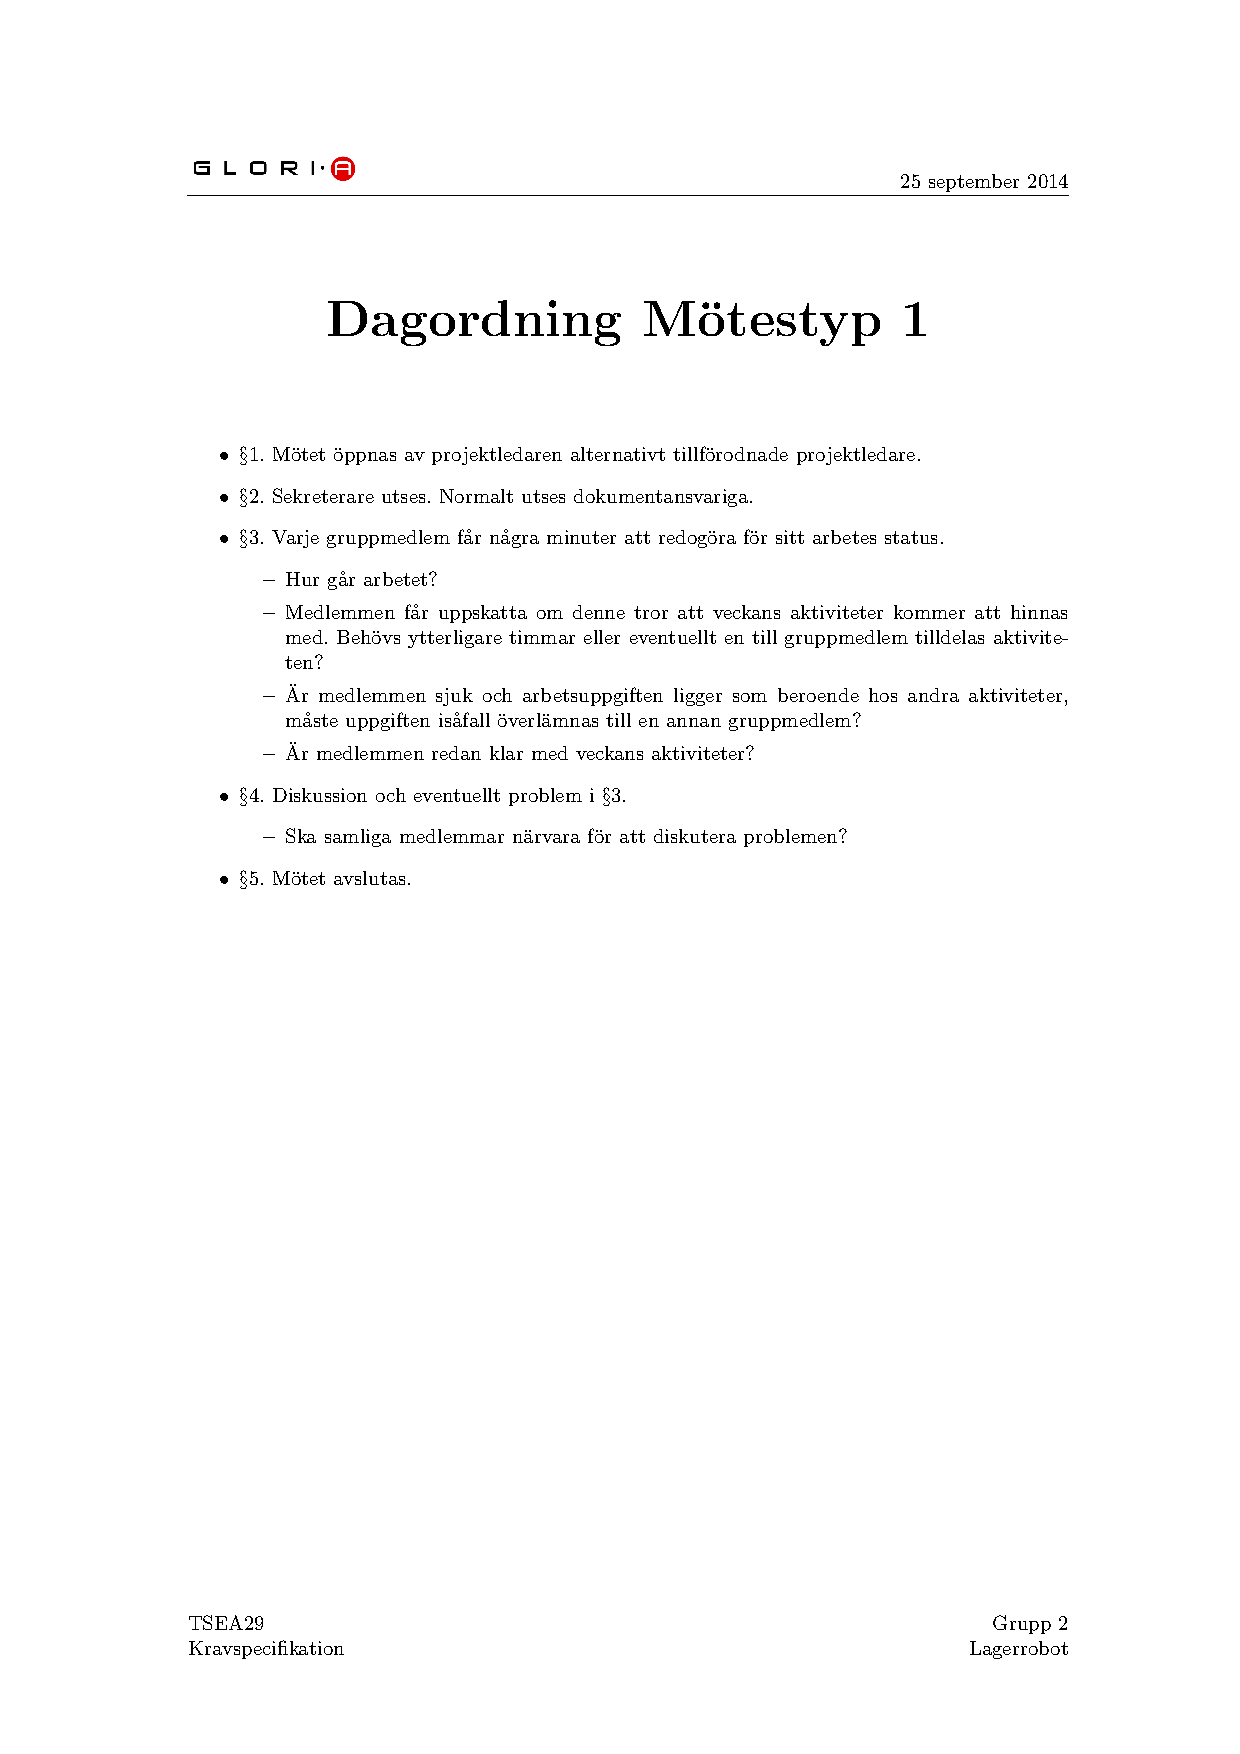
\includepdf[pages=-]{../motesprotokoll/motesmall1.pdf}

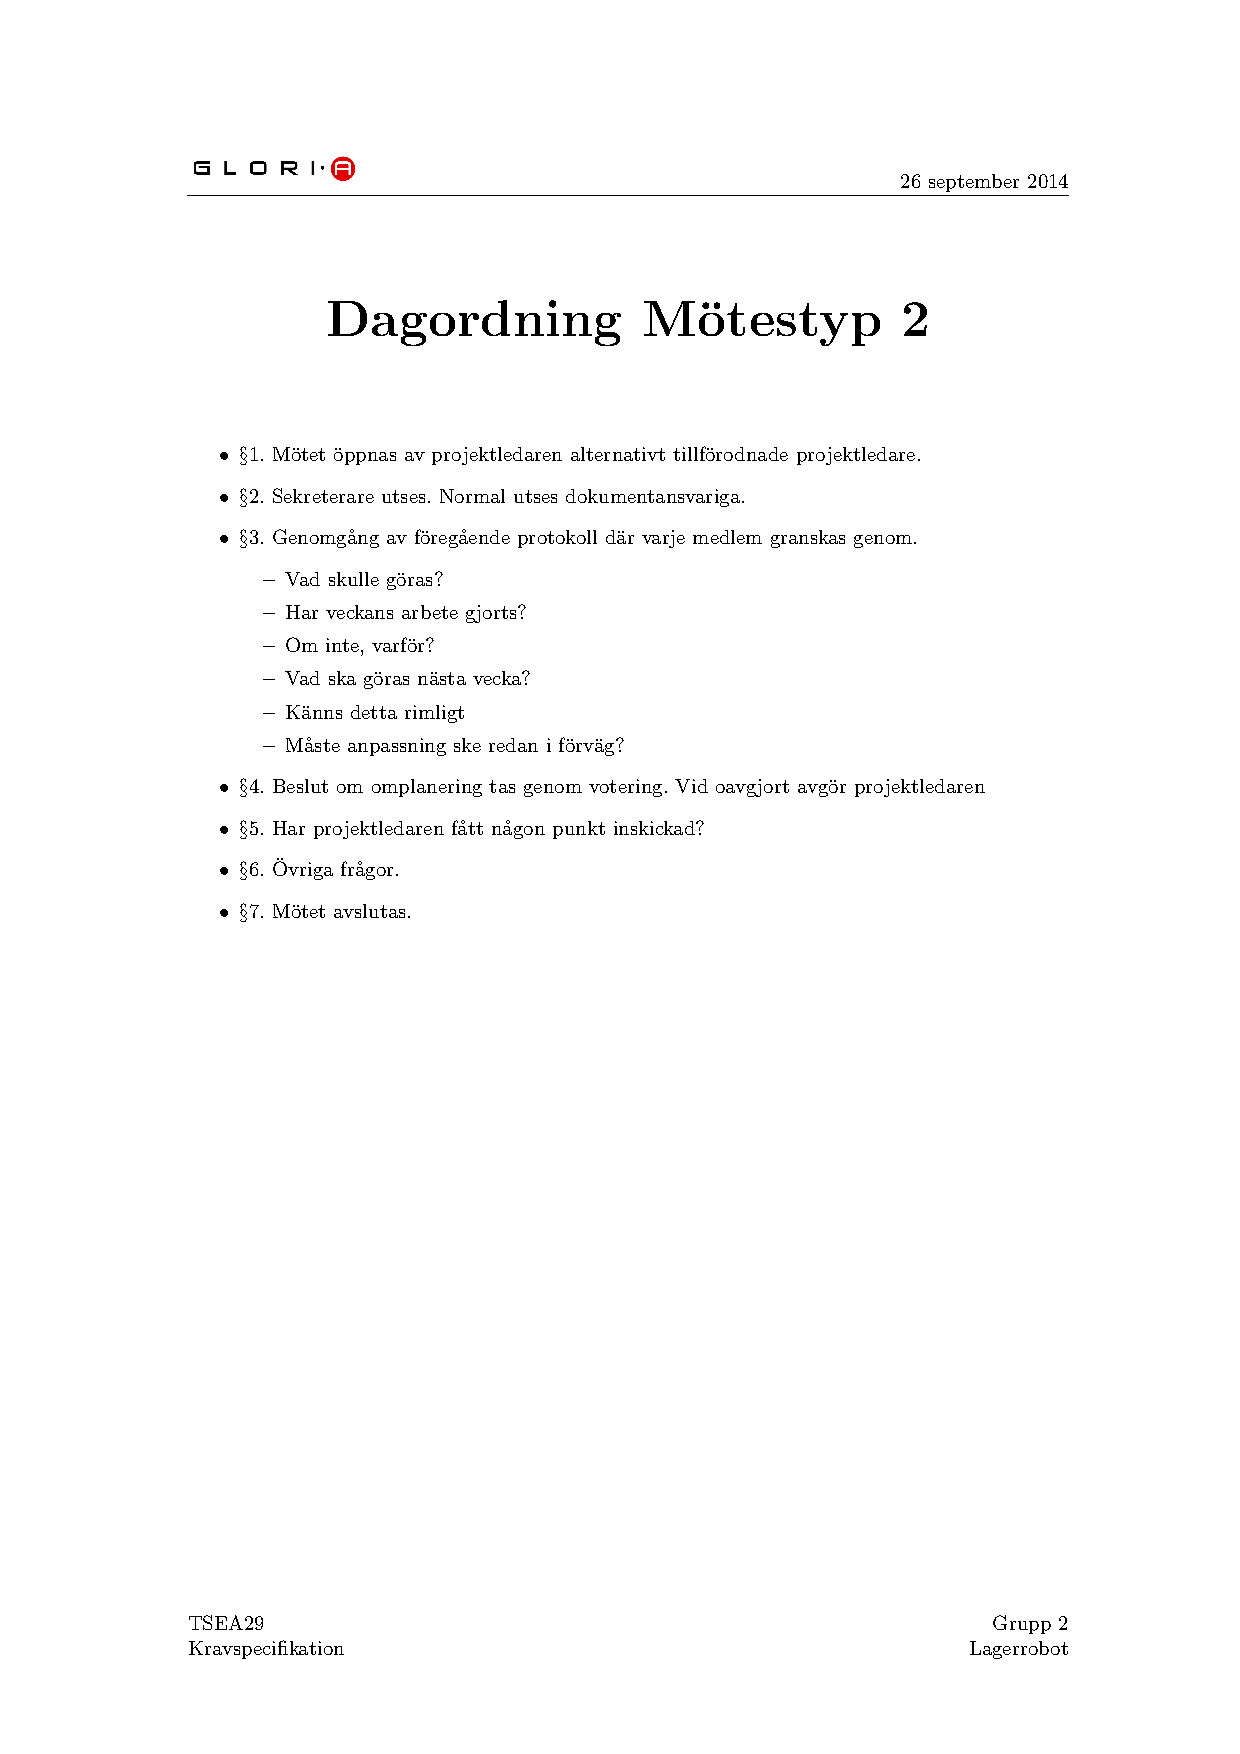
\includepdf[pages=-]{../motesprotokoll/motesmall2.pdf}


\newpage
\section{Tidsplan} \label{ap:tidsplan}
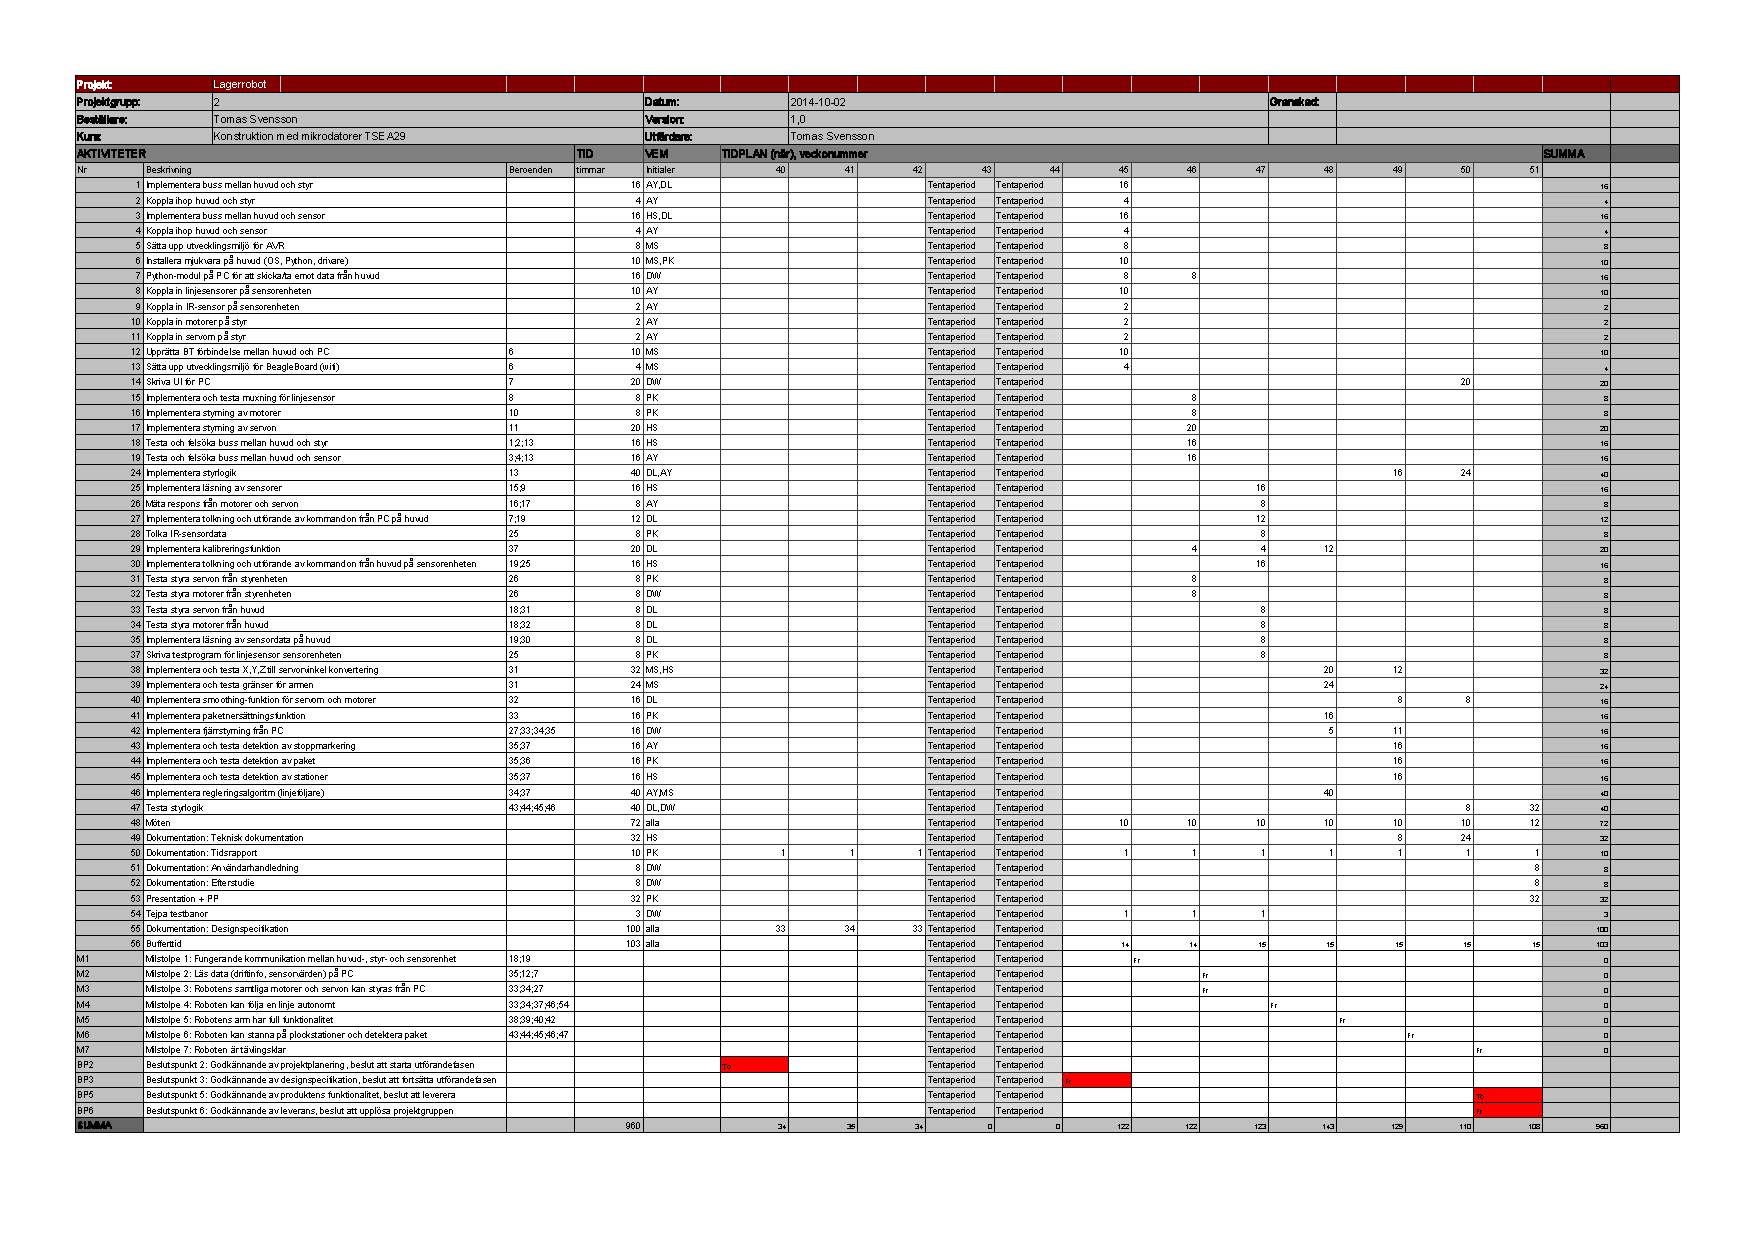
\includegraphics[angle=90, scale=0.7]{../tidsplan/tidsplan_v1.0.pdf}

\end{appendices}


\end{document}
